\documentclass[14pt]{article}
\usepackage{graphicx}

\title{\textbf{Tarea 02 - Lenguajes de Programación}}
\author{Navarro Meléndrez Erick Joel}
\begin{document}
	\maketitle
	En algunos problemas se pide escribir o responder preguntas, esto lo debes incluir en un documento "reporte.tex" implementado en TEX (o algúna descendiente) y "reporte.pdf" su versión compilada. Debe quedar extremadamente claro a qué problema corresponde cada parte del reporte.
	\\
	\\
	{\large\textbf{Problema 5}}
	\\ La llamada (bundle ’(”a” ”b” ”c”) 0) es un buen uso de bundle? ¿qué produce?
	¿por qué?
	\\
	\\\textit{La llamada no es un buen uso de \textbf{bundle} ya que esta entrada de datos hace que la función se cicle y nunca termine de ejecutar ningún proceso.
		\\EL motivo de esto es por que la función \textbf{drop} devuelve la misma lista de entrada al recibir como segundo argumento al 0. Por tanto, la lista no varia al llamar nuevamente a \textbf{bundle}, haciendo que esta sea llamada una y otra vez sin concretar nada.}
	\\
	\\{\large\textbf{Problema 9}}
	\\ Dibuja un diagrama como el de la figura anterior pero para la lista ’(11 9 2 18 12
	14 4 1).
	\\
	\begin{center}
		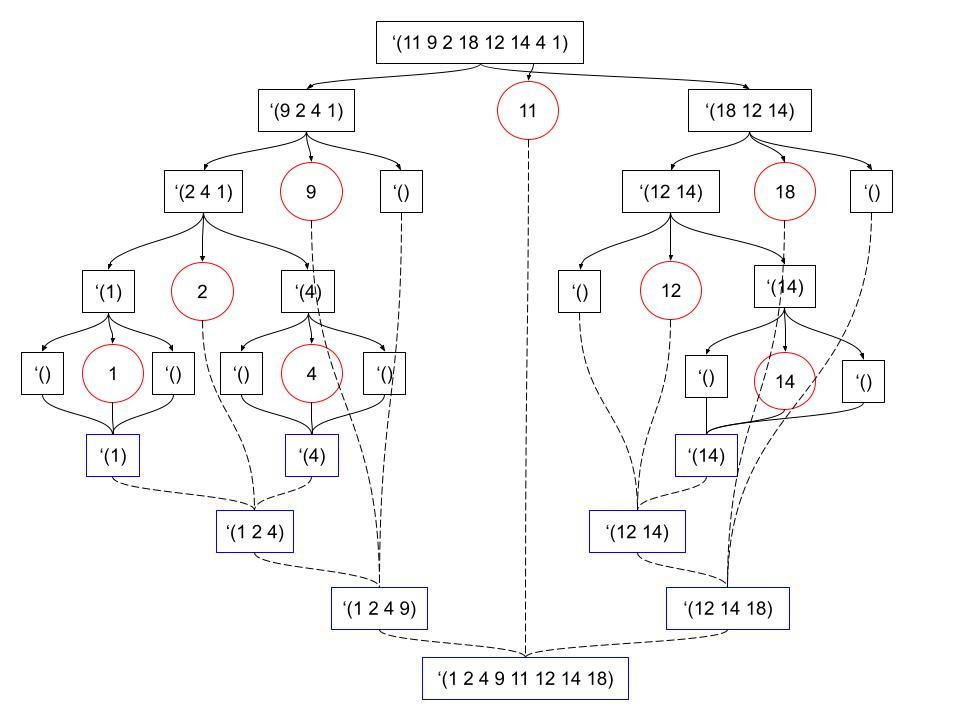
\includegraphics[width=0.8\textwidth]{Problema9}
	\end{center}
	{\large\textbf{Problema 11}}
	\\ Si la entrada a quicksort contiene varias repeticiones de un número, va a regresar
	una lista estrictamente más corta que la entrada. Responde el por qué y arregla el problema.
	\\
	\\\textit{Al aplicar \textbf{quicksort} a una lista de elementos repetidos, la función \textbf{quicksort} elimina los elementos repetidos por que los procedimientos \textbf{smallers} y \textbf{largers} toman únicamente los elementos estrictamente menores o mayores pero ignorando los que son iguales. Para solucionar este problema simplemente debemos crear un nuevo procedimiento llamado \textbf{equals} que devuelve la lista con todos los elementos iguales al pivote. Modificamos \textbf{quicksort} para que coloque esta lista entre la llamada de \textbf{largers} y \textbf{smallers}.}
	\\
	\\{\large\textbf{Problema 18}}
	\\ Considera la siguiente definición de \textbf{smallers}, uno de los procedimientos utilizados en \textbf{quicksort}, responde en qué puede fallar al utilizar esta versión modificada en el procedimiento de ordenamiento.
	\\
	\\\textit{Esta versión de \textbf{smallers} funciona y es capaz de capturar los resultados iguales a los pivotes pero al utilizarlo en \textbf{quicksort} hay un error que hace que la recursión se cicle indetemrinadamente y evite que el programa termine de ejecutarse.}
	\\
	\\{\large\textbf{Problema 19}}
	\\Escribe con tus propias palabras cómo funciona find-largest-divisor de gcd-structural. Responde por qué comienza desde (min n m).
	\\
	\\\textit{La función \textbf{find-largest-divisor} básicamente prueba caso por caso en orden descendente hasta encontrar	el valor que sea divisor común de m y n. El motivo por el cual comienza con '(min n m)' es por que el MCD siempre será menor o igual al más pequeño de los argumentos. Este también es el motivo por el cual prueba caso por caso en orden descendente.}
	\\
	\\{\large\textbf{Problema 20}}
	\\Describe con tus propias palabras cómo funciona find-largest-divisor de gcd-generative
	\\
	\\\textit{La función \textbf{find-largest-divisor} recibe dos números y establece el nuevo valor máximo como el viejo mínimo y al residuo de la división del viejo máximo y el viejo mínimo como el nuevo mínimo. Esto se realiza recursivamente hasta que se obtenga que el mínimo es 0, en ese momento se devuelve el último valor máximo que será el MCD.}
	\\
	\\{\large\textbf{Problema 22}}
	\\ Piensa y describe por qué no siempre es la mejor opción elegir el procedimiento más
	eficiente en tiempo de ejecución. Utiliza criterios que no sean el de "eficiencia".
	\\
	\\\textit{Aspirar a la eficiencia absoluta es contraproducente cuando realmente no ahorra una cantidad significativa de tiempo o espacio en nuestro programa o cuando su implementación es más difícil de leer que una no igual de eficiente pero más comprensible.}
	\\
	\\{\large\textbf{Problema 23}}
	\\Implementa un procedimiento que genere otro fractal, toma en consideración la discusión de esta tarea, caracteriza el tipo de recursividad que utilizaste y justifica la terminación de tu procedimiento.
	\\
	\begin{center}
		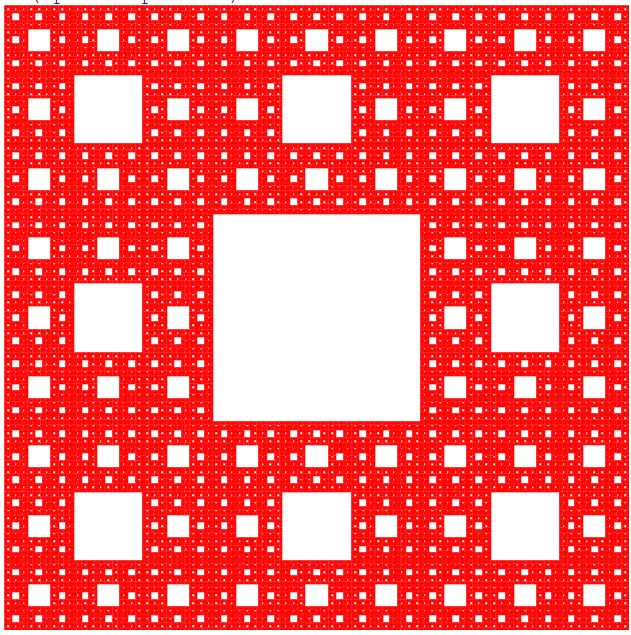
\includegraphics[width=0.8\textwidth]{spki}
	\end{center}
\end{document}